\subsection{Introducción al GIC}

Generalized Impedance Converter (GIC) son, como lo nombre lo indica, convertidores de impedancia, es decir para algunos filtros se podrá remplazar alguno de los componentes con un GIC. Por ejemplo cuando el uso de la bobina con inductancias de valor elevado puede involucrar agregar a un circuito un componente de gran tamaño como resistencia parásita indeseado, para ello, en rango de frecuencias donde se permite utilizar ampliadores operacionales, se utilizan los GIC.

Los GIC tienen la siguiente configuración:

\begin{figure}[h]
    \centering
    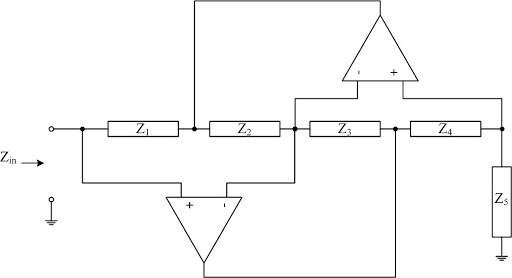
\includegraphics[scale = 0.7]{../Ejercicio1-FiltroConGIC/Informe/giccir.jpg}
    \caption{Generalized Impedance Converter Gen\'erico}
    \label{ej1gicnormal}
\end{figure}

Considerando los amplificadores ideales, o sea con $A_{vol} \longrightarrow \infty$ y $Z_{Ain} \longrightarrow \infty$ como no hay corriente entre $V^+ \hspace{0.1cm} V^-$ para ninguno de los operacionales, hay sólo tres corrientes, puesto que la corriente de $Z_2$ es la misma que la de $Z_3$, y la de $Z_4$ que la de $Z_5$ obtenemos que:
$$I_4 = \frac{Vin}{Z_5} \hspace{.5cm} I_2=\frac{I_1Z_1}{Z_2} \hspace{.5cm} I_2=\frac{I_4Z_4}{Z_3}$$
$$\therefore I_4 = I_1\frac{Z_1Z_3}{Z_2Z_4}$$
Por lo que la impedancia de entrada del GIC sera:
$$Z_{in} = \frac{Z_1 Z_3  Z_5}{Z_2  Z_4}$$
De esta manera es posible simular cualquier componente, sea resistivo capacitivo o inductivo mediante la selección adecuada de los componentes. Luego utilizando el GIC es posible obtener filtros de segundo orden como el notch, pasa-todo y pasa-banda minimizando el espacio utilizado. 

\subsection{Diseño de un Filtro Pasa-Todo}

Se implemento el siguiente circuito:

\begin{figure}[H]
    \centering
    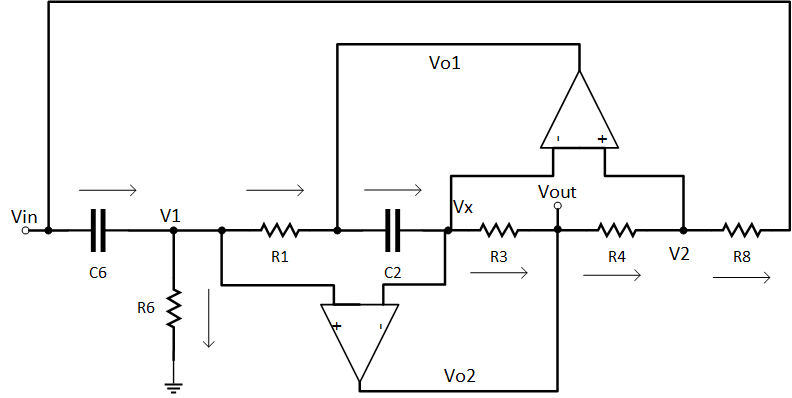
\includegraphics[scale = 0.7]{../Ejercicio1-FiltroConGIC/Informe/circuito.png}
    \caption{Circuito de un Filtro con GIC}
    \label{ej1cir}
\end{figure}

\subsubsection{Respuesta en frecuencia}\label{ej1resp}

Considerando que los amplificadores operacionales son ideales obtenemos que:

\begin{equation}
    \begin{split}
        &Vo1 = V1 - R1I_1 \hspace{1cm} Vo2 = Vx - R3I_3 \\
&Vo1 = Vx + \frac{1}{sC2}I_2 \hspace{.7cm} Vo2 = V2 + R4I_4  
    \end{split}
    \label{ej1eq1}
\end{equation}
 

\begin{equation}
    \therefore I_4 = I_1\frac{sC2R3R1}{R4}
    \label{ej1eq2}
\end{equation}

Además como $Avol \longrightarrow \infty$,

$$V1 = Vx = V2$$
$$I_1 = I_{C6} - I_{R6} \hspace{1CM} I_{C6} = (Vin - V1)sC6 \hspace{1cm} I_{R6} = \frac{V1}{R6}$$
$$I_{R8} = I_4$$

\begin{equation}
    \therefore Vx = Vin\frac{s^2C2C6R1R3R6R8 + R4R6}{sC2R1R3R8(sC6R6 + 1) + R4R6}
    \label{ej1eq3}
\end{equation}

Luego remplazando las ecuaciones (\ref{ej1eq2}) y (\ref{ej1eq3}) en (\ref{ej1eq1}) la función de transferencia quedará como:

\begin{equation}
    H(s) = \frac{Vout}{Vin} = \frac{s^2C2C6R1R3R6R8 - sC2R1R3R4 + R4R6}{s^2C2C6R1R3R6R8 + sC2R1R3R8 + R4R6}
    \label{ej1eq4}
\end{equation}

Esta respuesta en frecuencia corresponde a un Pasa-Todo con:

\begin{equation}
\label{ej1eq5}
    \omega_0 = \sqrt{\frac{R4}{C2C6R1R3R8}}
\end{equation}
\begin{equation}
\begin{split}
\label{ej1eq6}
    &Q_z = -R6 \sqrt{\frac{C6R8}{C2R1R3R4}} \\
    &Q_p = R6 \sqrt{\frac{C6R4}{C2R1R3R8}}    
\end{split}
\end{equation}

Se simplifica las ecuaciones si establecemos los valores de los componentes como la siguiente:

$$R1 = R3 = R4 = R8 = R$$
$$R6 = Q  R $$
$$C2 = C6 = C$$

Del cual modifica la transferencia como:

\begin{equation}
    \label{ej1eq7}
     H(s) = \frac{Vout}{Vin} = \frac{s^2C^2R^2 - s\frac{CR}{Q} + 1}{s^2C^2R^2 + s\frac{CR}{Q} + 1}
\end{equation}

\subsubsection{Funcionamiento de Resistencias}

\begin{itemize}
    \item Resistencia $R8$:
    
    La función de esta resistencia es es conectar la salida del GIC que le da un camino a la corriente y/o la suministra. Luego el efecto de esta resistencia en casos limites sera:
    $$\lim_{R8 \longrightarrow 0} H(s) = 1 - \frac{sC2R1R3}{R6}$$
    En esta circunstancia se comporta como un filtro pasa altos, donde la impedancia del $C2$ y $C6$ se vuelve despreciable y a su vez  circula mayor corriente en el GIC. Debido a esto aumenta la caída de tensión en los componentes resistivos del GIC, dando lugar a un incremento en la tensión de salida. 
    
    En caso de que R8 tenga un valor muy elevado:
    $$\lim_{R8\longrightarrow\infty} H(s) = \frac{sC6R6}{sC6R6 + 1}$$
    Es posible visualizar el circuito como abierto en la salida del GIC, es decir que no pasa corriente por ella. Es entonces que la tensión de salida $Vout = V1$, que tiene configuración de un RC pasa altos. 
    
    Cabe mencionar que para los valores límite de R8, el filtro deja de ser de segundo orden, con lo que su presencia es crucial para obtener los resultados esperados a la hora de utilizar un GIC para un filtro pasa-todo.
    
    \item Resistencia $R6$:
    
    Esta resistencia es de suma importancia ya que presenta un rol importante en la selección del factor de calidad $Q$, es decir los polos y los ceros del circuito. Manteniendo las otras resistencias fijas con valor R y los capacitores de valor C de modo que la única resistencia que varia es R6 obtenemos el siguiente gráfico del polo y ceros:
    
    \begin{minipage}{\textwidth}
    \centering
    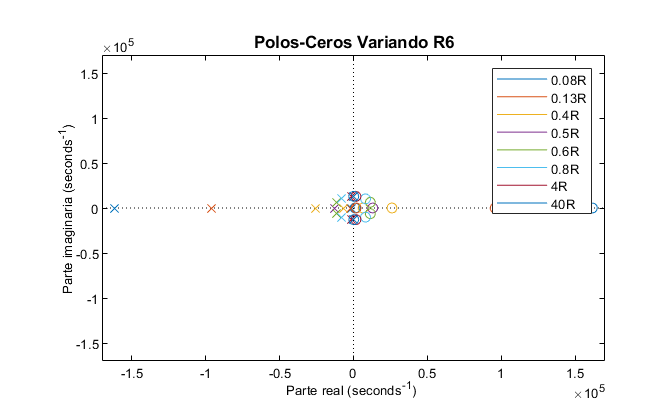
\includegraphics[scale = 0.8]{../Ejercicio1-FiltroConGIC/Informe/polor6.png}
    \end{minipage}
    \begin{minipage}{\textwidth}
    \centering
    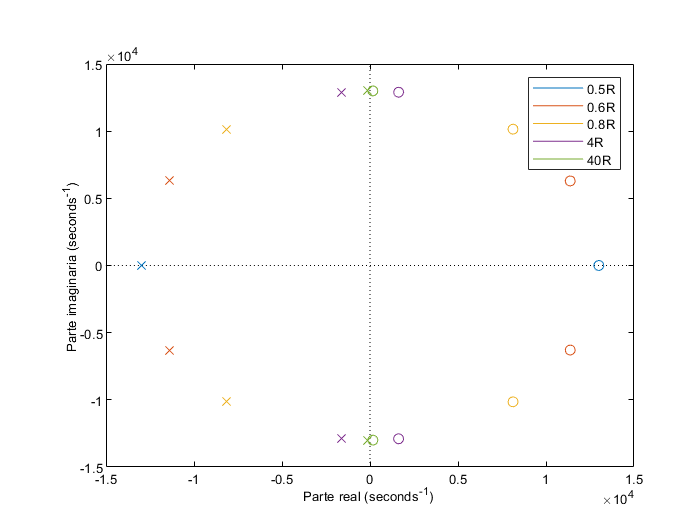
\includegraphics[scale = 0.7]{../Ejercicio1-FiltroConGIC/Informe/polor6-1.png}
    \captionof{figure}{Distribución de Polos y Ceros Variando R6}
    \end{minipage}
    
    Se nota entonces que los polos y ceros son opuestos para cualquier valor de R6. Además para valores mayores de Q, o sea valores mayores de $R6 = QR$, se acercan al eje imaginario sobre la circunferencia de radio $\omega_0$. Por lo que podemos apreciar que:
    $$\lim_{R8\longrightarrow\infty} H(s) = \frac{s^2C2C6R1R3R8 + R4}{s^2C2C6R1R3R8 + R4} = 1$$
    Cuya respuesta nos indica que al desconectar R6 el circuito deja pasar toda frecuencia sin cambio de fase, en esencia un cable. 
    
    En contra parte, valores pequeños de Q dejan de pertenecer a la circunferencia $\omega_0$, y se mueven en el eje real. Es claro si tomamos valores pequeños de R6 tenemos:
    $$\lim_{R8\longrightarrow 0} H(s) = -\frac{R4}{R8}$$
    Es equivalente entonces a un circuito de amplificación inversa con realimentación $R4$ y $R8$ en serie a la entrada. 
    
\end{itemize}

\subsubsection{Análisis de Sensibilidad}

Dado que en las experiencias se desea el menor error posible, se debe tomar en cuenta las tolerancias y los valores comerciales que restringen la elección de parámetros del circuito. Para ello se realiza un análisis de las sensibilidades
de los distintos parámetros con respecto a cada componente, esto indicara el peso que tendrá cada componente en el circuito. 

La sensibilidad se calcula como:
$$S^y_x = \frac{x}{y}\frac{dy}{dx}$$
Donde `$x$' es el componente e `$y$' la sensibilidad de un parámetro, que en este caso serán $\omega_0$, $Q_z$ y $Q_p$ dados por las ecuaciones \ref{ej1eq5} y \ref{ej1eq6}. Entonces para cada uno de los componentes su sensibilidad sera:

\begin{table}[H]
	\centering
	\begin{tabular}{|c||c|c|c|c|c|c|c|}
		\hline
		$y/x$ & $R_1$          & $C_2$          & $R_3$          & $R_4$         & $R_8$          & $C_6$          & $R_6$ \\ \hline \hline
		\\[-1em]
		$\omega_0$                                 & $-\nicefrac{1}{2}$ & $-\nicefrac{1}{2}$ & $-\nicefrac{1}{2}$ & $\nicefrac{1}{2}$ & $-\nicefrac{1}{2}$ & $-\nicefrac{1}{2}$ & 0     \\ \hline
		\\[-1em]
		$Q_z$                                        & $-\nicefrac{1}{2}$ & $-\nicefrac{1}{2}$ & $-\nicefrac{1}{2}$ & $-\nicefrac{1}{2}$ & $\nicefrac{1}{2}$ & $\nicefrac{1}{2}$  & 1     \\ \hline
		$Q_p$                                        & $-\nicefrac{1}{2}$ & $-\nicefrac{1}{2}$ & $-\nicefrac{1}{2}$ & $\nicefrac{1}{2}$ & $-\nicefrac{1}{2}$ & $\nicefrac{1}{2}$  & 1     \\ \hline
	\end{tabular}
	\caption{Sensibilidad de los componentes}
\end{table}

Cabe notar que se verifica la propiedad de suma:
$$\sum_n R_n^y - \sum_k C_k^y = 0$$

De acuerdo con las sensibilidades obtenidas, se sabe que las variaciones en $R6$ no tiene efecto en $\omega_0$, sin embargo presentan un rol importante para la selección de $Q_z$ y $Q_p$ dado que una modificación de esta afecta con una relación 1:1, o sea si se aumenta un porcentaje la resistencia se incrementa el valor de los $Q$ a la misma razón. Por otro lado, los otros componentes tienen una relación de modulo $\frac{1}{2}:1$ para $\omega_0$, $Q_z$ y $Q_p$. Pero dependiendo del signo de sensibilidad la variación positiva de una no necesariamente significa la elevación de las variables, por ejemplo en $\omega_0$ el aumento del valor de $R4$ causa que la variable se incremente, no obstante un aumento en el valor del resto de los componentes provoca un decremento de éste parámetro. 

\subsubsection{Impedancia del Circuito}

\begin{itemize}
    \item Impedancia de Entrada
    
    La impedancia de entrada de un circuito esta definida como:
    $$Zin = \frac{Vin}{Iin}$$
    Como se analiza el amplificador en condiciones ideales, su impedancia de entrada es infinita. Por lo que podemos obtener la corriente de entrada como:
    $$Iin = I_{C6}+I_{R8}$$
    Por lo tanto desde las relaciones de corrientes obtenidas en el ítem \ref{ej1resp} tenemos que:
    \begin{equation}
        Zin = \frac{Vin}{Iin} = \frac{s^2C2C6R1R3R6R8 + sC2R1R3R8 + R4R6}{s^2C2C6R1R3R8 + sC2R1R3} 
    \end{equation}
    Observando entonces que si se excita el circuito con tensión continua o frecuencias bajas su impedancia es muy alta. Este fenómeno es debido a los capacitores $C2$ y $C6$ que a estas frecuencias son componentes de alta impedancias, por lo que es escasa la corriente entrante al circuito. 
    
    \item Impedancia de Salida
    
    Como se espera trabajar en condiciones próximo al ideal, el amplificador operacional presenta muy baja impedancia de salida, por ende para nuestro circuito se espera tener una muy baja impedancia de salida aproximando el 0. 
\end{itemize}

\subsubsection{Implementación del Circuito}

Los filtros pasa-todo son utilizados para corregir la fase de una frecuencia en particular, de tal manera que modifica lo menos posible las demás frecuencias. Para ello, se selecciona la frecuencia de corte de los polos y ceros, de modo que a la frecuencia deseada ocurra un desfasaje de $180^o$. 

Para este filtro en particular se pide que:

\begin{table}[h]
\centering
\begin{tabular}{ccc}
\hline
$\omega_0${[}rad/s{]} & Q & Ganancia {[}dB{]} \\ \hline
13 000        & 4 & 0                 \\ \hline
\end{tabular}
\end{table}

Por lo que desde la función de transferencia dada por la ecuación \ref{ej1eq7} se sabe que:
$$\omega_0 = \frac{1}{RC}$$
Entonces obtenemos la relación que deben tener los componentes del circuito como:
$$RC = 76. 92\mu s$$
$$R6 = 4R$$

Se selecciono entonces una resistencia $R = 2.2k\Omega$ para realizar un análisis experimental, por lo que los componentes a utilizar serán:
\begin{table}[H]
	\centering
	\begin{tabular}{|c|c|c|c|}
		\hline
		           		& Valor ideal                              & Valor aplicado                      	& Error ($\%$) 	\\ \hline \hline
		$R_1$      		& $2.2k\Omega$                        & $2.2k\Omega$                       	& 0            	\\ \hline
		$C_2$      		& $34.965nF$				& $34.812nF$               		& 0.44         	\\ \hline
		$R_3$      		& $2.2k\Omega$                        & $2.2k\Omega$                       & 0            	\\ \hline
		$R_4$      		& $2.2k\Omega$                        & $2.2k\Omega$                       & 0            	\\ \hline
		$R_8$      		& $2.2k\Omega$                        & $2.2k\Omega$                       & 0            	\\ \hline
		$C_6$      		& $34.965nF$ 				& $34.812nF$               		& 0.44         	\\ \hline
		$R_6$      		& $8.8k\Omega$                      	& $8.9k\Omega$       			& 1.12            	\\ \hline
	\end{tabular}
	\caption{Valores de los Componentes Ideales y Aplicados}
\end{table}
Luego si experimentamos el circuito se notara en teoría:
\begin{table}[h]
\centering
\begin{tabular}{cc}
\hline
$\omega_0${[}rad/s{]} & Q    \\ \hline
13 057        & 4.05 \\ \hline
\end{tabular}
\end{table}

\subsubsection{Elección de Amplificador Operacional}

La selección de los amplificadores operacionales dependen del circuito a implementar, ya que son los que determinan que características son las mas importantes para el caso.

Para el filtro a aplicar se busca un gran GBW y $A_vol$ para el $A_vol(j\omega)$ no baje por los polos dominantes que actúan a frecuencias altas, de esta manera el integrado puede actuar cercano la ideal. En particular los filtros pasa-todos, que se utiliza para la corrección de fase, es importante que tenga ganancia de $0dB$ para toda frecuencia, por ello se debe mantener el mayor rango posible de frecuencia sin distorsiones. 

Otra de las características a considerar es el slew-rate, que al estar operando a altas frecuencias un alto valor de ella evita la posibilidad de que se vea limitada la tensión máxima a frecuencias menores menor al del polo. 

Por ultimo, la impedancia de entrada del amplificador operacional debe ser muy alta en relación con los otros componentes del circuito, es por esta que impide que circule corriente por las entradas del amplificador haciendo valida las ecuaciones realizadas anteriormente. 

Por lo tanto se tuvo en cuenta los opamps $LM833$ y $TL082$ las cuales cumplen con un considerable GBW, slew-rate y impedancia de entrada. Se selecciono entonces el $TL082$, que si bien tiene menor GBW que el $LM833$, a frecuencias que se utiliza el circuito $4MHz$ es suficiente por lo que luego se aprecio mas el slew-rate que es $13\frac{V}{\mu s}$ mayor al del $LM833$. 

\subsection{Análisis de Resultados}

\subsubsection{Respuesta en Frecuencia}

Realizando un análisis en frecuencia, superponiendo resultados teóricos, simulados y experimental se obtuvo el siguiente gráfico:

\begin{figure}[H]
    \centering
    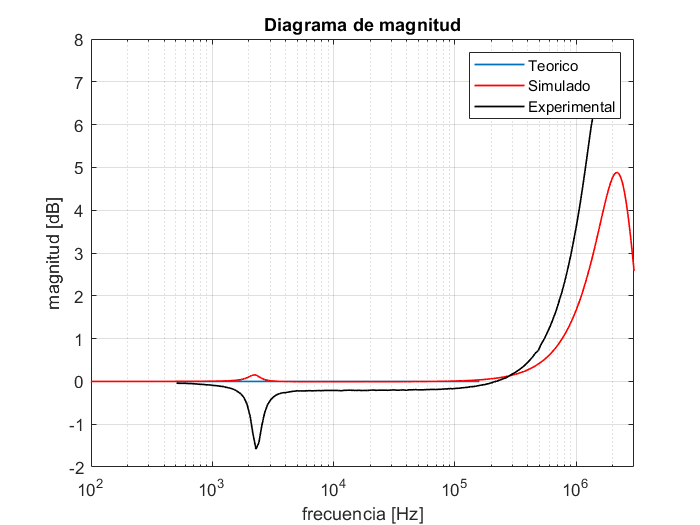
\includegraphics[scale = 0.7]{../Ejercicio1-FiltroConGIC/Informe/rfmag.png}
    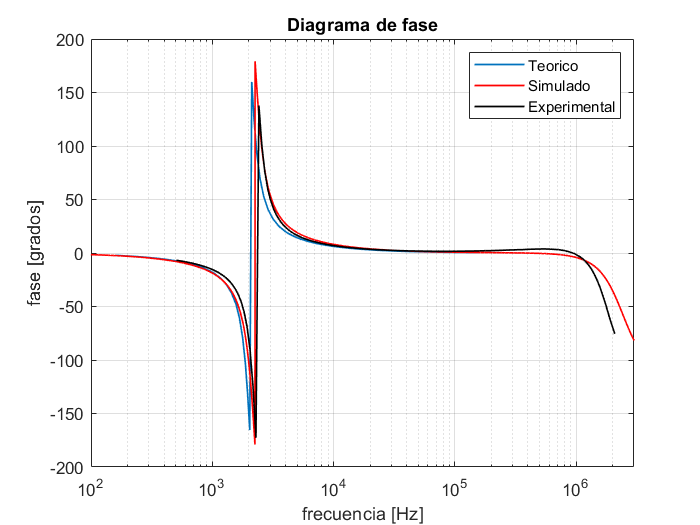
\includegraphics[scale = 0.7]{../Ejercicio1-FiltroConGIC/Informe/rfpha.png}
    \caption{Respuesta en Frecuencia del Circuito}
    \label{ej1rf}
\end{figure}

De esta notamos que en la frecuencia de corte $f_c = \frac{1}{2\pi}\omega_0 \approx 2.07kHz$ ocurre un cambio de fase de $-180^o$, si bien experimentalmente se obtuvo que su frecuencia de corte fue en $2.30kHz$. Esta leve diferencia es atribuido a las tolerancias de los componentes utilizados, resistencias de $5\%$ y capacitores de $20\%$. Además, la caída notoria en la frecuencia de corte es debido a que la transferencia presenta ceros y polos de orden 2 a una misma frecuencia, y ambos factores de calidad $Q > 1/\sqrt{2}$, es decir que son suficientemente grandes para provocar sobre-picos o sobre-caídas. El valor de $Q_p$ determinaría la magnitud de un sobre-pico en casos donde no hubiera ceros, mientras que el valor de $Q_z$ provocaría una sobre-caída. En otras palabras, si los valores del $Q_p$ y $Q_z$ son distintos en alguna frecuencia provocaría una subida o una caída dependiendo de sus valores. En nuestro caso, dado que se observa una caída, se concluye que los valores de $Q_z$ y $Q_p$ fue alterado por las dispersiones de los componentes, llevando que el valor de $Q_z$ sea mayor al de $Q_p$ en esta frecuencia. Estos fenomenos son observables el en la figura \ref{ej1despha}.

\begin{figure}[h]
    \centering
    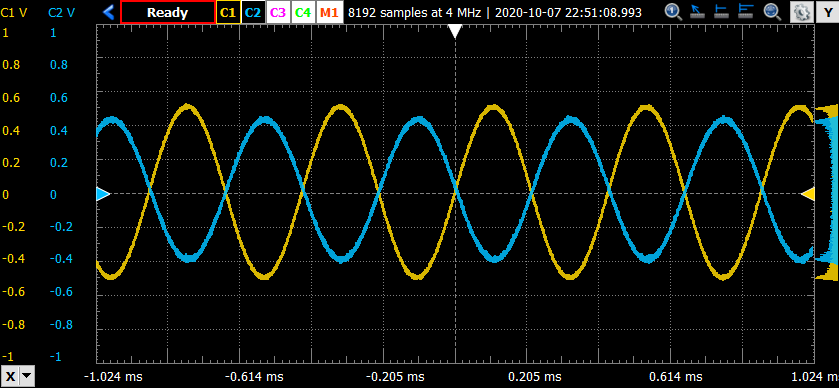
\includegraphics{../Ejercicio1-FiltroConGIC/Informe/desphaOsc.png}
    \caption{Respuesta en Frecuencia de 2.29kHz}
    \label{ej1despha}
\end{figure}

Por otro lado, en altas frecuencias, mayores a $200kHz$, se observa un sobre-pico ya que a partir de estas frecuencias comienzan a afectar los efectos del polo del operacional, que no se tuvieron en cuenta en el análisis teórico realizado anteriormente. A su vez, la diferencia en el sobre-pico es influenciado por las tolerancias de los componentes y las puntas de osciloscopio colocados al circuito, que inyectan una resistencia y capacitancia parásita al circuito, modificando en cierta medida la ubicación y la magnitud. 

\subsubsection{Impedancia de Entrada}

Para la medición de esta característica del circuito se coloco una resistencia en serie a la entrada del circuito, luego calculando la corriente que circula por la misma se tiene que la impedancia del circuito es $Zin = \frac{Vcarga}{i_{R1}}$. Para la selección la resistencia de testeo se utilizo uno cercano a los valores esperados de la impedancia de entrada, ya que si se pusiese una resistencia muy chica, la diferencia entre las tensiones medidas sobre sus bornes ser\'ia muy chica aumentando incertidumbre, y si se colocase una resistencia muy grande, la tensi\'on que caer\'ia ser\'ia mucho mayor a la que caer\'ia en el circuito, haciendo que la tensi\'on luego de la resistencia sea muy chica haciendo que sea mas vulnerable al ruido.

Luego la impedancia de entrada al circuito dado resulta en:

\begin{figure}[h]
    \centering
    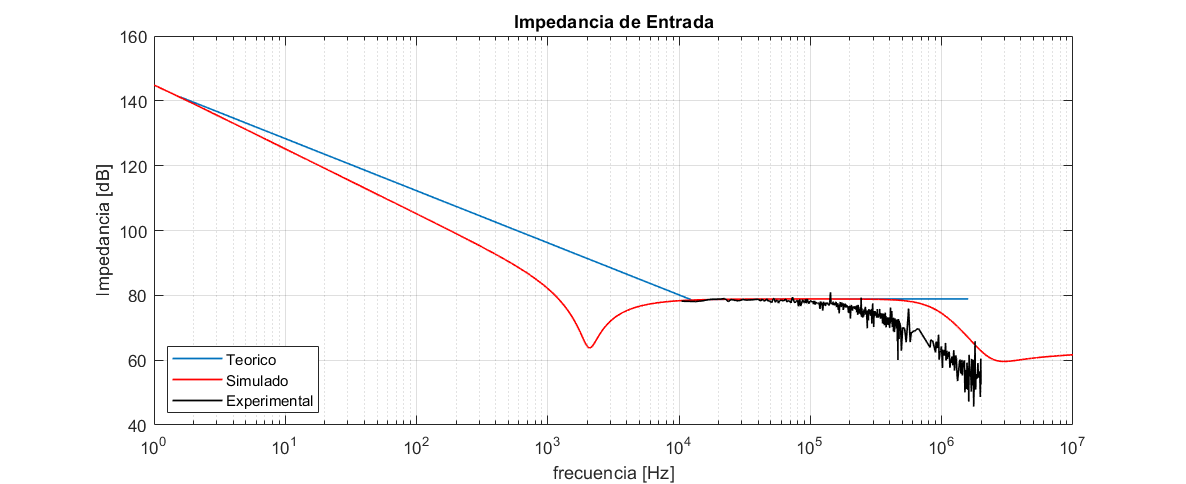
\includegraphics[scale = 0.6]{../Ejercicio1-FiltroConGIC/Informe/zin.png}
    \caption{Impedancia de Entrada del Circuito}
    \label{ej1zin}
\end{figure}

Observamos entonces que la impedancia de entrada a bajas frecuencias en muy alta debido a los capacitores del circuito. Luego de una caída por el cero, el módulo de la impedancia queda estable en las cercanías de $10k\Omega$ hasta que hacen efecto los polos dominantes de los operacionales en cercanía a $1MHz$. 

Cabe notar que a altas frecuencias porque sus tensiones de salida son bajas, el ruido es comparable con las señal de entrada, lo que logra inyectarse en las mediciones dando lugar a un grado de incertidumbre apreciable.

\subsubsection{Impedancia de Salida}

Para la medición de esta, se realizo la midió la salida del circuito en el vació y luego con una carga la salida. Como la corriente de salida debe ser la misma en el vació como en el de carga obtenemos que la impedancia de salida es:
$$Zout = R_{test} \frac{V_{test}}{V_{vacio} - V_{test}}$$
Luego su impedancia de salida resulto:

\begin{figure}[H]
    \centering
    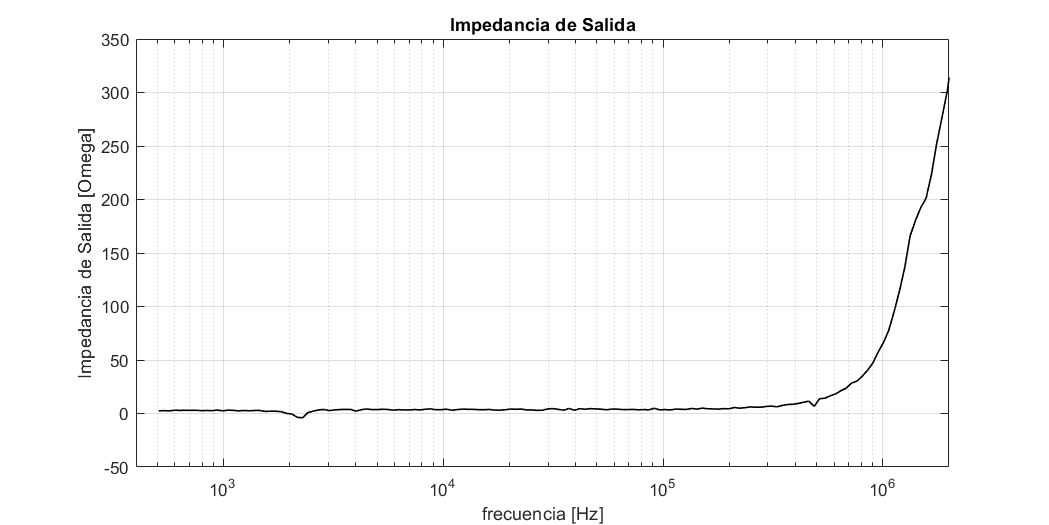
\includegraphics[scale = 0.6]{../Ejercicio1-FiltroConGIC/Informe/zout.png}
    \caption{Impedancia de Salida del Circuito}
    \label{ej1zout}
\end{figure}

Este resultado fue acorde a lo esperado, teniendo su impedancia para frecuencias menores a $1MHz$ aproximadamente iguales a 0. Se nota que para frecuencias mayores a $1MHz$ comienza a tomar otros valores, esto es debido a que los efectos de los polos en en el amplificador están tomando efecto en el circuito causando que los amplificadores ya no actúen de forma ideal.

\subsection{Respuesta al Escalón}

La transferencia del circuito $H(s)$ con $Q_p>\frac{1}{2}$ tiene característica de una oscilación subamortiguado, es decir que la estabilización temporal sufre una oscilación hasta que se pueda estabilizar. 

Este efecto es visible excitando el circuito con un escalón del cual la salida sera:
$$Y(s) = H(s)X(s) \hspace{.5cm} X(s) = \frac{1}{s}$$
Por lo que la respuesta al escalón es:
$$Y(s) = \frac{s^2C^2R^2 - s\frac{CR}{Q} + 1}{s^2C^2R^2 + s\frac{CR}{Q} + 1} \frac{1}{s}$$
Luego, obtenemos que:
$$y(t) = \frac{2 C R (e^{t (-\frac{\sqrt{-C^2 (4 Q^2 - 1) R^2}}{(2 C^2 Q R^2)} - \frac{1}{(2 C Q R)})} - e^{t (\frac{\sqrt{-C^2 (4 Q^2 - 1) R^2}}{(2 C^2 Q R^2)} -\frac{1}{(2 C Q R)})})}{\sqrt{-C^2 (4 Q^2 - 1) R^2)}} + 1$$
Donde obtenemos que $\omega_d = \sqrt{\omega_0^2 - \alpha^2}$ y $\alpha = \frac{1}{2CQR}$, luego $\omega_d = 12.9 \frac{rad}{s}$ y $\tau = \frac{1}{\alpha} = 615\mu s$.

Entonces la respuesta al escalón sera:

\begin{figure}[H]
    \centering
    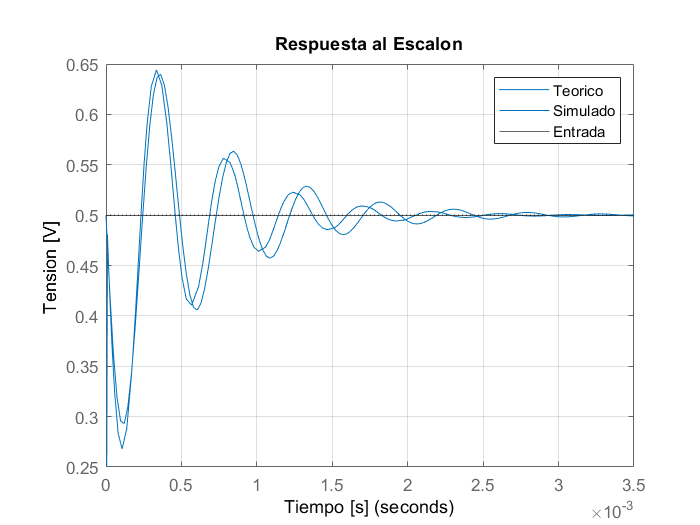
\includegraphics[scale = 0.8]{../Ejercicio1-FiltroConGIC/Informe/re.png}
    \caption{Respuesta al Escalón Teórico y Simulado}
    \label{ej1reteo}
\end{figure}

Del cual obtuvimos experimentalmente lo siguiente:

\begin{figure}[H]
    \centering
    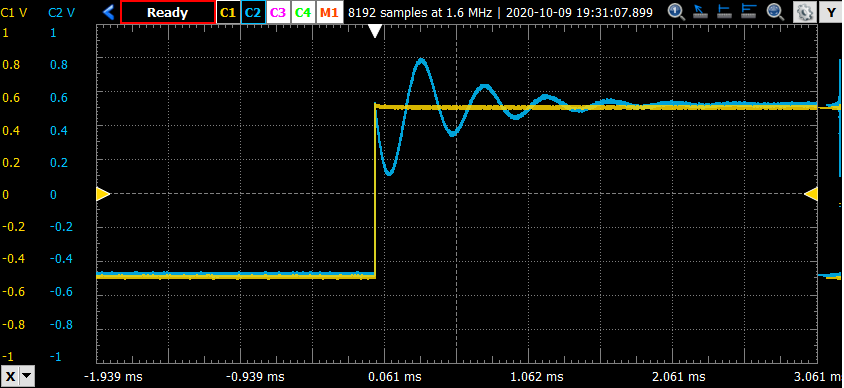
\includegraphics[scale = 0.8]{../Ejercicio1-FiltroConGIC/Informe/re1.png}
    \caption{Respuesta al Escalón Experimental}
    \label{ej1reexp}
\end{figure}

Se observa que las oscilaciones empiezan con pendiente negativa, lo que indica defasaje de 180 grados. Esto se debe al desfasaje introduce el filtro a las componentes de la cuadrada de frecuencia mayor a la de corte. Como las componentes de la cuadrada que actúan primero son las de mayor frecuencia, éstas se ven desfasadas 180 grados. 

Por otro lado, se establece el circuito a partir del quito pseudoperiodo, es decir que tiene un tiempo de establecimiento de aproximadamente $2.06ms$ en el experimental mientras que en la simulación y el teorico se establece a tiempos mayores al rededor de los $2.15ms$. Dado que existen resistencias parásitas dentro del circuito, es esperable esta mayor atenuación en la experiencia hecha.

Este tiempo de establecimiento es un problema para un filtro pasa-todo ya que a frecuencias con periodos menores a la misma los resultados obtenidos de la misma serán oscilantes en vez de la salida sea otra señal cuadrada. Por ejemplo para señales de frecuencia $1kHz$ o periodo $1ms$, la tension de salida resulta:

\begin{figure}[H]
    \centering
    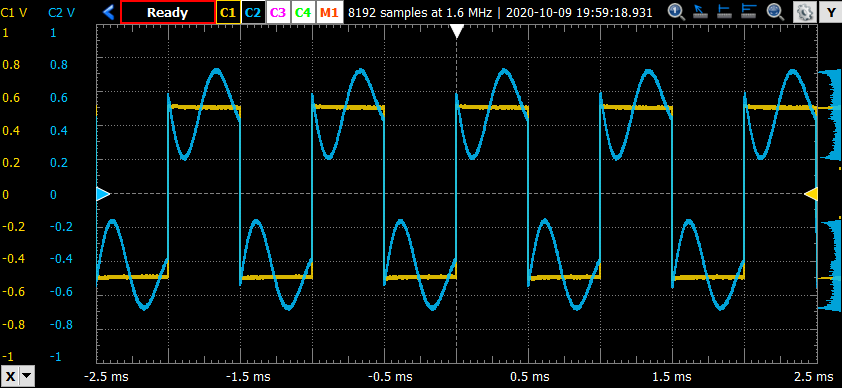
\includegraphics[scale = 0.8]{../Ejercicio1-FiltroConGIC/Informe/re1k.png}
    \caption{Respuesta al Escalon a 1kHz}
    \label{ej1re1k}
\end{figure}

\subsection{Limitaciones del Circuito}

Es importante tener en cuenta las características del amplificador operación a la hora de experimentar un circuito, es por ello que se deben saber los limites en la que podemos operar el circuito con funcionamiento normal. 

\subsubsection{Limitación por Tensión}

Debido a que los operacionales se alimentaron con $V_{CC} = \pm 9V$, si se excita el circuito con $18V_{pp}$ la salida se satura. Como lo podemos notar en la siguiente figura \ref{ej1limt}.

\begin{figure}[H]
    \centering
    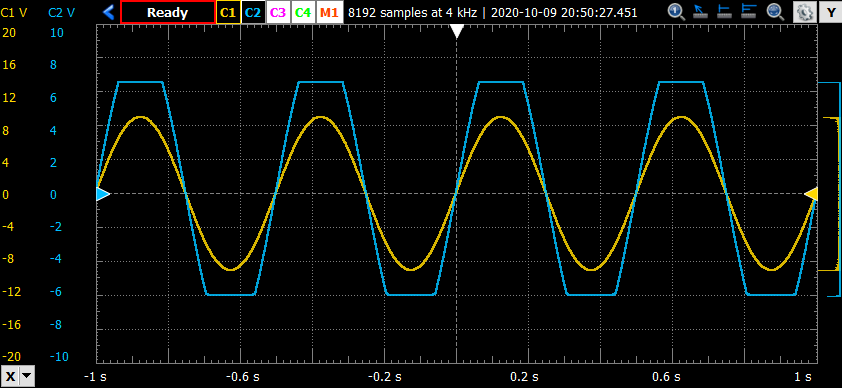
\includegraphics[scale = 0.8]{../Ejercicio1-FiltroConGIC/Informe/limtensionpng.png}
    \caption{Limite por Tensión}
    \label{ej1limt}
\end{figure}

Como se puede observar el circuito se satura a $12V_{pp}$, es decir que no permite que la tensión de entrada supere $12V_{pp}$, pues sino los resultados obtenidos no serán precisos.

\subsubsection{Limitación por Frecuencia}

El ancho de banda del operacional utilizado es de $4MHz$. Sin embargo, en las mediciones de respuesta en frecuencia se pone de manifiesto que el polo del operacional afecta el comportamiento del filtro mucho antes, como se observa en los gr\'aficos de la figura \ref{ej1rf}. Por lo tanto, s\'olo puede asegurarse que el filtro siga el comportamiento calculado hasta los $200kHz$ donde luego de ello aparece el sobre-pico.

\subsubsection{Limitación por Señal}

En caso de utilizar el circuito con entrada no sinusoidales, es importante tener en cuenta el tiempo de establecimiento de la respuesta temporal, que es de $2.06ms$. 

\subsection{Conclusión}

Con el uso de un GIC, se pudo implementar un pasa-todo, si bien con cierto grado de error debido a tolerancias y/o componentes parásitas, se obtuvo a grandes rázagos los resultados esperados hasta los $200kHz$, donde pasando esta frecuencia el operacional deja de tener carácter ideal. Es también importante remarcar la importancia de sensibilidad que tienen los componentes, es decir debemos tener en cuenta cuales son los componentes mas importantes a la hora de realizar una experiencia para tener resultados acorde a lo planeado, pues una variación de ciertos componentes puede afectar ampliamente los resultados obtenidos. 